\documentclass[12pt]{article}
\usepackage[paperwidth=40in, paperheight=40in, margin=1in]{geometry}
\usepackage{tikz}
\usepackage{tcolorbox}
\usepackage{xcolor}
\usepackage{parskip}
\usepackage{lmodern}
\usetikzlibrary{positioning}

% Fonts & layout
\renewcommand{\familydefault}{\sfdefault}

% === Font Size Control Macro ===
\newcommand{\PosterFontSize}{\fontsize{45}{50}\selectfont}

% Box styling
\tcbset{
	colframe=black!30!white,
	colback=gray!5!white,
	boxrule=0.5pt,
	arc=1mm,
	top=4pt, bottom=4pt,
	left=6pt, right=6pt,
	width=0.48\textwidth,
	height=0.20\textheight,
	valign=center,
	fontupper=\PosterFontSize
}

% Space macros
\newcommand{\HVI}{\textbf{H\textsuperscript{6}}}
\newcommand{\GVI}{\textbf{G\textsuperscript{6}}}
\newcommand{\SVI}{\textbf{S\textsuperscript{6}}}
\newcommand{\PVI}{\textbf{P\textsuperscript{3}}}
\newcommand{\CIII}{\textbf{C\textsuperscript{3}}}

% a,b,c as base vectors of unit cells
\newcommand{\va}{\ensuremath{\mathbf{a}}}
\newcommand{\vb}{\ensuremath{\mathbf{b}}}
\newcommand{\vc}{\ensuremath{\mathbf{c}}}
\newcommand{\vd}{\ensuremath{\mathbf{d}}}
\begin{document}
	
	\begin{center}
		{\fontsize{90}{100}\selectfont\textbf{Unit Cells in Space or Spaces for Unit Cells}}\
		
		
		
		\ [0.5cm]
		{\fontsize{60}{60}\selectfont Lawrence C. Andrews and Herbert J Bernstein — ACA 2025}
	\end{center}
	
	\vspace{0.8cm}
	
	% Row 1 — Tree and Abstract
	\noindent
	\parbox[t]{0.48\textwidth}{
		\tcolorbox[title=Crystallographic Space Map]
		\begin{center}
			\scalebox{2.}{
				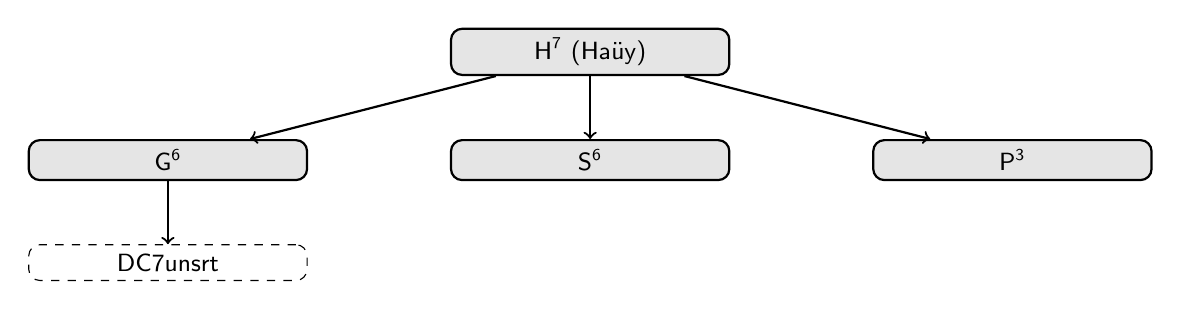
\begin{tikzpicture}[
					node distance=0.8cm and 1.8cm,
					measurement/.style={text width=3.3cm, align=center, rectangle, draw=black,
						fill=gray!20, rounded corners, font=\small, thick},
					symmetry/.style={text width=3.3cm, align=center, rectangle, draw=black,
						dashed, fill=white, rounded corners, font=\small}
					]
					\node[measurement] (H7) {H\textsuperscript{7} (Ha\"uy)};
					\node[measurement] (G6) [below left=of H7] {G\textsuperscript{6}};
					\node[measurement] (S6) [below=of H7] {S\textsuperscript{6}};
					\node[measurement] (P3) [below right=of H7] {P\textsuperscript{3}};
				%	\node[symmetry] (C3) [below=of S6] {C\textsuperscript{3}};
					\node[symmetry] (DC7) [below=of G6] {DC7unsrt};
					\draw[->, thick] (H7) -- (G6);
					\draw[->, thick] (H7) -- (S6);
					\draw[->, thick] (H7) -- (P3);
				%	\draw[->, thick] (S6) -- (C3);
					\draw[->, thick] (G6) -- (DC7);
				\end{tikzpicture}
			}
		\end{center}
		\endtcolorbox
	}
	\hfill
	\parbox[t]{0.48\textwidth}{
		\tcolorbox[title=Abstract]
		Crystallographers describe unit cells using multiple mathematical spaces, each revealing different aspects of geometry, symmetry, or classification. But they don't think about them as spaces. \\ Beginning with conventional parameters in \HVI{}, we trace transformations through \GVI{} and \SVI{} into polar (\PVI{}), and geometric (DC7unsrt) spaces. Keep in mind
		that another common description is as the 3 base vectors
		of the conventional unit cell, \va, \vb, \vc; this is 
		also a space, a 3-dimensional space of 3-D Euclidiean  vectors.
		\endtcolorbox
	}
	
	\vspace{1cm}
	
	% Row 2 — HVI and GVI
	\noindent
	\parbox[t]{0.48\textwidth}{
		\tcolorbox[title=\HVI{} – Conventional Parameter Space]
		\textbf{Conventional Parameter Space (\HVI{})}
		
		Six coordinates: $a$, $b$, $c$, $\alpha$, $\beta$, $\gamma$. 
		Not ideal for comparing geometry or symmetry directly.
		("H" was chosen to honor Ren\'e Just Ha\"uy, often described as 
		the first modern crystallographer.)
		\endtcolorbox
	}
	\hfill
		\parbox[t]{0.48\textwidth}{
		\tcolorbox[title=\CIII{} – Character Space]
		\textbf{Why do we need spaces for unit cells?}
		
		\HVI is inconvienent for describing the differences between unit cells/lattices, and there is no obvious method to display cells'
		relationships. Besides, other spaces are already in use; they are
		simply not always described as spaces. Representing cells as points
		in a space allows the simple application of the techniques of
		linear algebra.
		\endtcolorbox
	}
	
	\vspace{1cm}
	
	% Row 3 — SVI and PVI
	\noindent
	\parbox[t]{0.48\textwidth}{
		\tcolorbox[title=\SVI{} – Selling/Delone Space]
		\textbf{Delone Space (\SVI{})}
		
		For a unit cell with base vectors \va, \vb, \vc,
		and -\vd = -\va-\vb-\vc, a vector in \SVI~ is defined as 
		[\ensuremath{\vb \cdot \vc}, \ensuremath{\va \cdot \vc}, \ensuremath{\va \cdot \vb},
		 \ensuremath{\va \cdot \vd}, \ensuremath{\vb \cdot \vd}, \ensuremath{\vc \cdot \vd}]
		. In \SVI, the subspace of the Selling/Delaunay reduced points is a convex region. 
		The Bravais types form linear manifolds. The region of the reduced vectors has only 6 boundaries,	simplifying analyses. \\
		\SVI is actually the space that
		Selling/Delaunay reduction is performed in.
		\endtcolorbox 
	}
	\hfill
	\parbox[t]{0.48\textwidth}{
	\tcolorbox[title=\GVI{} – Niggli Space]
	\textbf{Niggli Space (Metric Tensor Space) (\GVI{})}
	)
		For a unit cell with base vectors \va, \vb, \vc,
		a vector in \GVI~ is defined as 
	[\ensuremath{\va \cdot \va}, \ensuremath{\vb \cdot \vb}, \ensuremath{\vc \cdot \vc},
	\ensuremath{2\vb \cdot \vc}, \ensuremath{2\va \cdot \vc}, \ensuremath{2\va \cdot \vb}]. \GVI is the basis for Niggli reduction. The domain of Niggli-reduced
	cells is non-convex with complex boundary behavior, so distance
	calculations can be done, but they can be complex.
	\endtcolorbox
}

	
	\vspace{1cm}
	
	% Row 4 — DC7 and Character Space
	\noindent
	\parbox[t]{0.48\textwidth}{
		\tcolorbox[title=DC7unsrt – Dirichlet 7\, unsorted]
		\textbf{Seven-Dimensional Dirichlet derived (DC7unsrt)}
		
		Seven scalars derived from Voronoi cells. Focuses on geometric relationships and symmetry inference.
		Bernstein, Andrews, and Xerri, Acta Cryst A79 (2005). 369-380. Experience shows
		that distance calculations in this space can be fast.
		\endtcolorbox
		
		
		
		
		
	}
	\hfill
	\parbox[t]{0.48\textwidth}{
	\tcolorbox[title=\PVI{} – Polar Space]
	\textbf{Polar Space (\PVI{})} \\
	\PVI is defined as the space of 3 polar coordinates, [\ensuremath{
	(|\va|,\alpha), 
	(|\vb|,\beta), 
	(|\vc\,\gamma)}]. \\
	\PVI has a conceptual advantage that is it more directly related to the 
	unit cell parameters that are commonly used in crystallography 
	(\HVI{}). Polar coordinates are often converted to x,y, Euclidean 
	coordinates for simple calculations with commensurate measures, so distance calculations make sense.
	 Because they are in Angstrom units, they are more
	familar. 
	\endtcolorbox
}

	
\end{document}
